\chapter*{\FontH{\Huge Der weisse Adler}}
\addcontentsline{toc}{chapter}{Der weisse Adler}
\lettrine[lines=3]{\color{red}J}{a}, Johann war eitel. Ihr werdet sagen, dass das nicht schön ist, aber so ganz unrecht hatte er nicht. Schön war er schon, der Johann. Denn Johann war der einzige weisse Adler weit und breit. Die anderen waren braun oder grau, wie Adler eben so sind. Auch schön, aber nicht so speziell wie Johann und oft ist es ja gerade das Spezielle, was wir als besonders schön oder manchmal auch als besonders hässlich empfinden. Und die anderen Adler mussten zugeben, dass das besonders reine Weiss seiner Federn tatsächlich sehr schön war. Und so nahm es Johann niemand übel, dass er so eitel war. 

Johann tat das aber gar nicht gut. Er wurde beinah von Tag zu Tag ein bisschen eitler. 

\enquote{Ha, ihr seht ja alle so schmutzig aus, mit euren braunen Federn, als ob ihr gerade in den Dreck gefallen wärt.} rief er den anderen zu. Aber auch das war schon bald unter seiner Würde. Mit nach oben geschobenem Schnabel zog er seine Kreise in der Luft. Erhaben fühlte er sich und auserwählt vom Schicksal. Mit Verachtung blickte er auf die anderen Adler herab. Es dauerte nicht lange, da redete er sich sogar ein, der König der Adler zu sein. Und so benahm er sich auch.

Eigenartig war, dass die anderen Adler ihm glaubten. Sie dachten, weil Johann so Einzigartig aussah, müsse er wohl auch etwas besonderes sein. Und wer so besonders ist, ist sicher dazu bestimmt, der König zu sein. Also brachten sie ihm Mäuse, wenn er Hunger hatte und erfüllten ihm auch sonst alle Wünsche. Ein paar wenige Adler, die ihm besonders viele Mäuse brachten, standen in der Gunst von Johann weit oben. Sie bekam zur Belohnung von ihm eine weisse Feder geschenkt. Und weil Johann die nur selten verschenkte, waren die die eine hatten, auch etwas besonderes und genossen bei den anderen Adlern hohes Ansehen. 

So ging es einige Jahr ganz gut. Johann war der König, er hatte seine treuen Freunde und konnte regieren wie er wollte. Nicht dass er das sehr ausgenutzt hätte. Eigentlich war er nur etwas faul und liess sich gerne bedienen. Hochnäsig zog er seine Kreise am Himmel.

Ein Adler-Sprichwort sagt, dass wer hoch steigt, auch tief fällt. Das habt ihr vielleicht schon einmal gehört, bei uns Menschen gibt es das ja auch. Und so erging es auch Johann. Eines Tages kam er auf die Idee, dass ein König auch einen Thron brauche. Aber was wäre denn gut genug, ein Thron für den König der Lüfte zu sein? Die Sonne war zu heiss. Der Mond war zwar schön, aber mal war er gross und rund und dann wurde er immer schmaler. Das passte Johann gar nicht und auch das blasse Gelb gefiel ihm nicht. Als mal jemand vorgeschlagen hatte, er möge sich doch auf eine Wolke setzten, war er beleidigt.

\begin{figure}[hb]
\centering
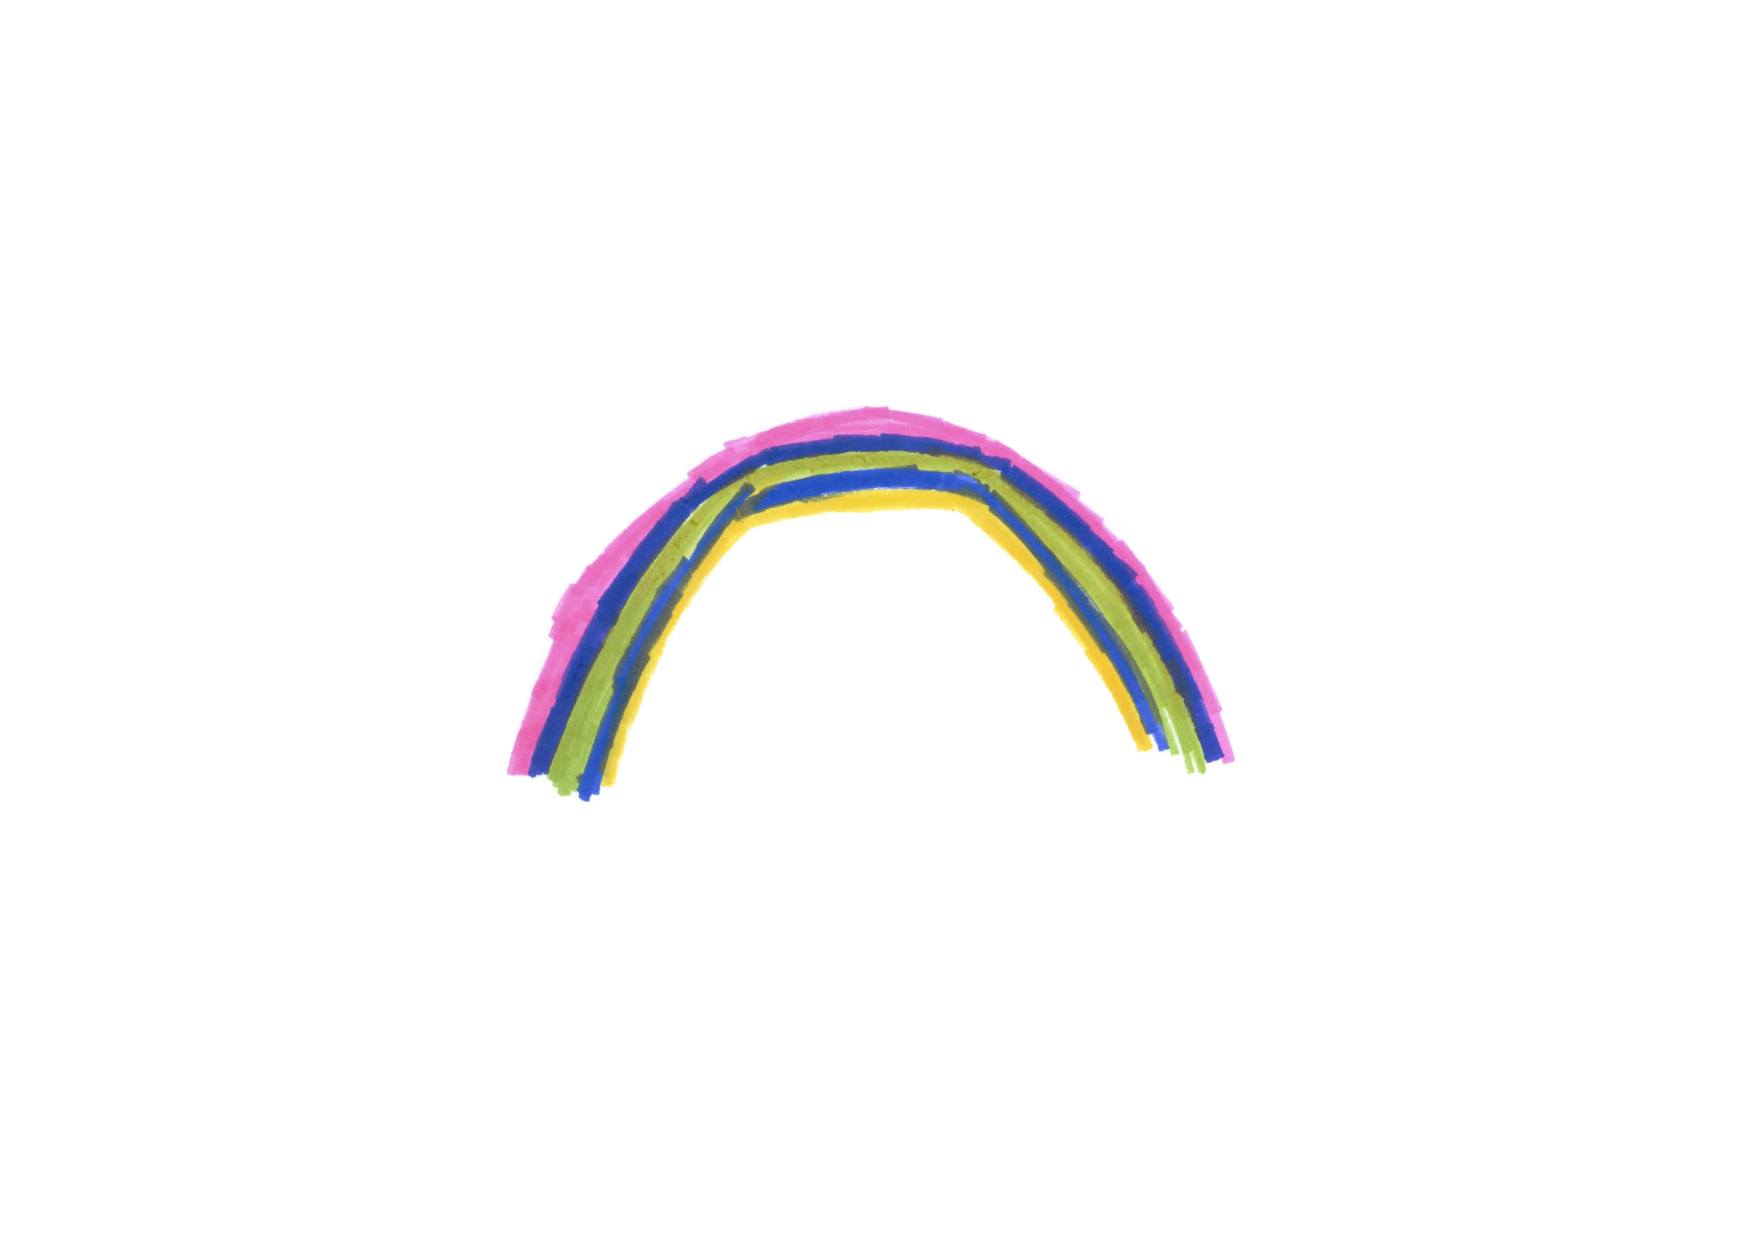
\includegraphics[width=.7\textwidth]{bilder/adler.pdf}
\end{figure}

\enquote{Die Wolken sind für den gemeinen Adler, nicht aber für ihren König.} Und so blieb nur der Regenbogen übrig. Der war aber auch besonders gut geeignet! Die herrlich leuchtenden Farben passten wunderbar zu den weissen Federn unseres Johann. 

Zufrieden mit seiner Wahl beäugte Johann den Regenbogen von allen Seiten und beschloss, dass hier sein Thron sein soll. So lud er alle Adler und auch die anderen Vögel des Himmels ein, Zeugen seiner feierlichen Thronbesteigung zu sein. Niemand traute sich die Einladung abzulehnen, immerhin war Johann ja der König. Und so putzte sich alles, was fliegen kann heraus und versammelte sich um den Regenbogen.

Johann, zufrieden so viele Bewunderer zu haben, plusterte sich nochmals gewaltig auf, flog bis an den höchsten Punkt des Regenbogens und setzte sich.

\enquote{Auf den Regenbogen setzten?} höre ich euch fragen. Da habt ihr Recht, natürlich geht das nicht. Ein Regenbogen besteht nur aus Licht und auf Licht kann man sich nicht setzen. Ihr wisst das, aber Johann wusste das nicht! Und so plumpste er direkt durch den Regenbogen durch. Alle Adler und alle Vögel fingen an zu lachen. Und das Schlimmste war, der Regebogen hatte das weisse Federkleid unseres Johann ganz verfärbt. Hier ein roter Streifen, dort violette Tupfer und dazu überall gelbe und grüne Sprengsel. So sehr Johann auch flatterte und zappelte, de Farbe wollte nicht abgehen. Ja, wieder war Johann etwas besonderes, aber nicht mehr von der schönen Sorte.

\enquote{Hahaha, da kommt ja unser Fasnachts-Johann} riefen die anderen Vögel, \enquote{Der sieht ja aus wie ein Clown.} Und dabei blieb es. Vorbei war die Zeit vom König Johann. Niemand brachte ihm mehr Mäuse wenn er Hunger hatte, niemand putzte sein Federkleid und bewundert wurde er auch von niemandem mehr. Seine einstigen Freunde vermieden es, mit ihm gesehen zu werden. Die weisse Feder, die er ihnen geschenkt hatte, versteckten sie im Wald. Keiner wollte erinnert werden, einmal so einen bunten Vogel bedient zu haben. 

Und es wurde sogar immer schlimmer für ihn. Schon riefen die ersten anderen Adler:

\enquote{Hey, Fastnachst-Johann, bring uns Mäuse, wir haben Hunger} und fingen an, auf ihn einzupicken. Da blieb Johann nichts anderes übrig, als jetzt für die anderen Adler Mäuse zu suchen. Ein elendes Leben hatte er. Alle kommandierten ihn jetzt herum, so wie er sie einst kommandiert hatte. Das war nicht länger auszuhalten, beschloss er. Er konnte auch einfach nicht mehr. Er hatte keine Kraft mehr und es wurden zu viele Demütigungen.

Und so machte er sich auf den Weg und flog davon. Nach Norden flog er, weil ihm gerade nichts anderes einfiel. Weiter flog er und immer weiter, bloss weg von den anderen Adlern, immer höher in den Norden, wo nur Schnee und Eis sind und keine anderen Adler mehr wohnen. So kam Johann in das Reich der Schneekönigin.

Als die unseren Johann sah, freute sie sich. Denn ihr müsst wissen, dass am Nordpol -- und gerade da war unser Johann -- alles weiss ist. Überall nur Schnee und Eis. Kein Baum, kein Strauch und schon gar keine Blume oder sonst etwas, dass nicht weiss ist. Und so freute sich die Schneekönigin sehr, als unser bunter Johann geflogen kam. 

\enquote{Gute Tag, Johann} sagte sie. Und nach einem langen Blick: 

\enquote{Wie schön Du bist.} 

\enquote{Ach, wenn es nur wahr wäre.} seufzte Johann und erklärte: 

\enquote{Es ist noch gar nicht lange her, da war ich der Schönste Adler unter der Sonne. Rein und weiss gerade so wie der Schnee hier. Sogar König bin ich gewesen, weil ich so rein war. Aber ich wurde überheblich und hab nicht Recht getan. Ich bin faul geworden und habe mich füttern lassen. Und dann wollte ich zum König aller Vögel werden und vom Regenbogen aus regieren. Da bin ich gefallen. Meine Federn haben sich verfärbt wie ein Hemd beim Waschen und alle haben mich verstossen. So haben mich die Winde zu Dir geblasen.}

Die Schneekönig verstand, dass Johann aufrichtig bereut hat und es ihm Leid tat, so überheblich gewesen zu sein. Da küsste sie ihn auf die Stirn. Ganz zart und vorsichtig. Hätte sie ihn mehr geküsst, wäre Johann sofort erfroren, denn alles, was die Schneekönigin berührt, wird sofort zu Eis. 

Ein eiskalter Schauer erfasste Johann. Noch nie hatte er so gefroren. Seine Flügel wurden steif und er konnte sich kaum bewegen. Die Federn wurden hart, als wären sie aus Glas. Ein paar brachen nur schon durch den Wind. Aber auch die Reste des Regenbogens in seinen Federn gefroren. Und sobald er sich ein bisschen erholt hatte und sich etwas besser bewegen konnte, fielen sie klirrend auf den kalten Boden.

Johann war glücklich. Er verbeugte sich zum Dank tief vor der Schneekönigin, breitete die Flügel aus und flog wieder zurück in den Süden. Dort lebte er von nun an als Adler unter Adlern. Weiss zwar und anders als die anderen, aber weder besser noch schlechter als sie. \hfill {\color{red}\decofourleft}
